\documentclass{article}
\usepackage[margin=1in]{geometry}
\usepackage{amsmath,amsthm,amssymb}
\usepackage{bbm,enumerate,mathtools}
\usepackage{tikz,pgfplots}
\usepackage{chessboard}
\usepackage[hidelinks]{hyperref}
\usepackage{multicol} % Problem 35

\newenvironment{question}{\begin{trivlist}\item[\textbf{Question.}]}{\end{trivlist}}
\newenvironment{note}{\begin{trivlist}\item[\textbf{Note.}]}{\end{trivlist}}
\newenvironment{references}{\begin{trivlist}\item[\textbf{References.}]}{\end{trivlist}}
\newenvironment{related}{\begin{trivlist}\item[\textbf{Related.}]\end{trivlist}\begin{enumerate}}{\end{enumerate}}


\begin{document}
\rating{3}{2}
Let a $k$-tile \textit{multipolyform} be a generalized polyform on a tiling,
that is, a choice of $k$ tiles in the tiling that are edge-adjacent.
\begin{figure}[ht!]
  \centering
  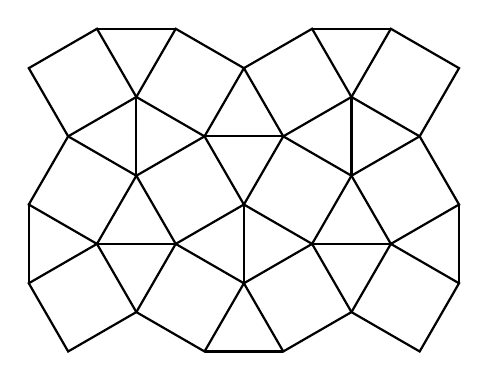
\begin{tikzpicture}
    \foreach \x/\y in {0/0, 0/2, 1/1, 2/0, 2/2, 3/1} {
      \draw[thick] ({\x * (0.5 + sqrt(3)/2) + 1}, {\y * (0.5 + sqrt(3)/2)})--
            ({\x * (0.5 + sqrt(3)/2) + 1 + sqrt(3)/2},{\y * (0.5 + sqrt(3)/2) + 0.5})--
            ({\x * (0.5 + sqrt(3)/2) + 1.5 + sqrt(3)/2},{\y * (0.5 + sqrt(3)/2) + 0.5 - sqrt(3)/2})--
            ({\x * (0.5 + sqrt(3)/2) + 1.5}, {\y * (0.5 + sqrt(3)/2) - sqrt(3)/2})--cycle;
    }

    \foreach \x/\y in {0/0, 1/-1, 1/1, 2/0, 3/-1, 3/1} {
      \draw[thick] ({\x * (0.5 + sqrt(3)/2) + 1}, {\y * (0.5 + sqrt(3)/2)  + 1})--
            ({\x * (0.5 + sqrt(3)/2) + 1.5}, { \y * (0.5 + sqrt(3)/2) + 1 + sqrt(3)/2})--
            ({\x * (0.5 + sqrt(3)/2) + 1.5 + sqrt(3)/2}, {\y * (0.5 + sqrt(3)/2) + 0.5 + sqrt(3)/2})--
            ({\x * (0.5 + sqrt(3)/2) + 1 + sqrt(3)/2}, {\y * (0.5 + sqrt(3)/2) + 0.5})--cycle;
    }
    \foreach \x/\y in {0/0, 1/1, 2/0, 3/1, 4/0} {
      \draw[thick] ({1 + \x * (0.5 + sqrt(3)/2)}, {0 + \y * (0.5 + sqrt(3)/2)})--
            ({1 + \x * (0.5 + sqrt(3)/2)}, {1 + \y * (0.5 + sqrt(3)/2)});
    }

    \foreach \x/\y in {0/0, 0/2, 1/1, 1/-1, 2/0, 2/2} {
      \draw[thick] ({1 + sqrt(3)/2 + \x * (0.5 + sqrt(3)/2)}, {0.5 + \y * (0.5 + sqrt(3)/2)})--
            ({2 + sqrt(3)/2 + \x * (0.5 + sqrt(3)/2)}, {0.5 + \y * (0.5 + sqrt(3)/2)});
    }
  \end{tikzpicture}
  \caption{The snub square tiling.}
\end{figure}
\begin{figure}[ht!]
  \centering
  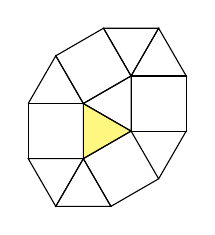
\begin{tikzpicture}[scale=0.7]
    \draw (0, 0) rectangle (1, 1);
    \draw[fill=yellow!50] (1, 0)--(1,1)--({1 + sqrt(3)/2},0.5)--cycle;
    \draw ({1 + sqrt(3)/2},1.5)--(1,1)--({1 + sqrt(3)/2},0.5)--cycle;
    \draw ({1 + sqrt(3)/2},1.5) rectangle ({2 + sqrt(3)/2},0.5);
    \draw ({1 + sqrt(3)/2},1.5)--(1,1)--(0.5, {1 + sqrt(3)/2})--({0.5 + sqrt(3)/2},{1.5 + sqrt(3)/2})--cycle;
    \draw (0,1)--(0.5, {1 + sqrt(3)/2})--(1,1);
    \draw ({1 + sqrt(3)/2},1.5)--({1.5 + sqrt(3)/2},{1.5 + sqrt(3)/2})--({2 + sqrt(3)/2},1.5)--cycle;
    \draw ({1 + sqrt(3)/2},1.5)--({0.5 + sqrt(3)/2},{1.5 + sqrt(3)/2})--({1.5 + sqrt(3)/2},{1.5 + sqrt(3)/2})--cycle;
    \draw (1, 0)--({1 + sqrt(3)/2},0.5)--({1.5 + sqrt(3)/2},{0.5 - sqrt(3)/2})--(1.5, {-sqrt(3)/2})--cycle;
    \draw (0, 0)--(0.5, {-sqrt(3)/2})--(1,0)--cycle;
    \draw (0.5, {-sqrt(3)/2})--(1,0)--(1.5, {-sqrt(3)/2})--cycle;
    \draw ({2 + sqrt(3)/2},0.5)--({1.5 + sqrt(3)/2},{0.5-sqrt(3)/2});%({2 + sqrt(3)/2},0.5);
  \end{tikzpicture}
  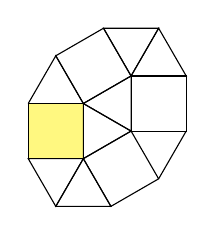
\begin{tikzpicture}[scale=0.7]
    \draw[fill=yellow!50] (0, 0) rectangle (1, 1);
    \draw (1, 0)--(1,1)--({1 + sqrt(3)/2},0.5)--cycle;
    \draw ({1 + sqrt(3)/2},1.5)--(1,1)--({1 + sqrt(3)/2},0.5)--cycle;
    \draw ({1 + sqrt(3)/2},1.5) rectangle ({2 + sqrt(3)/2},0.5);
    \draw ({1 + sqrt(3)/2},1.5)--(1,1)--(0.5, {1 + sqrt(3)/2})--({0.5 + sqrt(3)/2},{1.5 + sqrt(3)/2})--cycle;
    \draw (0,1)--(0.5, {1 + sqrt(3)/2})--(1,1);
    \draw ({1 + sqrt(3)/2},1.5)--({1.5 + sqrt(3)/2},{1.5 + sqrt(3)/2})--({2 + sqrt(3)/2},1.5)--cycle;
    \draw ({1 + sqrt(3)/2},1.5)--({0.5 + sqrt(3)/2},{1.5 + sqrt(3)/2})--({1.5 + sqrt(3)/2},{1.5 + sqrt(3)/2})--cycle;
    \draw (1, 0)--({1 + sqrt(3)/2},0.5)--({1.5 + sqrt(3)/2},{0.5 - sqrt(3)/2})--(1.5, {-sqrt(3)/2})--cycle;
    \draw (0, 0)--(0.5, {-sqrt(3)/2})--(1,0)--cycle;
    \draw (0.5, {-sqrt(3)/2})--(1,0)--(1.5, {-sqrt(3)/2})--cycle;
    \draw ({2 + sqrt(3)/2},0.5)--({1.5 + sqrt(3)/2},{0.5-sqrt(3)/2});%({2 + sqrt(3)/2},0.5);
  \end{tikzpicture}
  \hspace{1cm}
  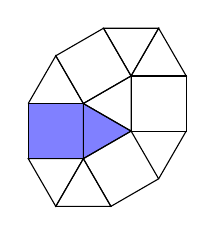
\begin{tikzpicture}[scale=0.7]
    \draw[fill=blue!50] (0, 0) rectangle (1, 1);
    \draw[fill=blue!50] (1, 0)--(1,1)--({1 + sqrt(3)/2},0.5)--cycle;
    \draw ({1 + sqrt(3)/2},1.5)--(1,1)--({1 + sqrt(3)/2},0.5)--cycle;
    \draw ({1 + sqrt(3)/2},1.5) rectangle ({2 + sqrt(3)/2},0.5);
    \draw ({1 + sqrt(3)/2},1.5)--(1,1)--(0.5, {1 + sqrt(3)/2})--({0.5 + sqrt(3)/2},{1.5 + sqrt(3)/2})--cycle;
    \draw (0,1)--(0.5, {1 + sqrt(3)/2})--(1,1);
    \draw ({1 + sqrt(3)/2},1.5)--({1.5 + sqrt(3)/2},{1.5 + sqrt(3)/2})--({2 + sqrt(3)/2},1.5)--cycle;
    \draw ({1 + sqrt(3)/2},1.5)--({0.5 + sqrt(3)/2},{1.5 + sqrt(3)/2})--({1.5 + sqrt(3)/2},{1.5 + sqrt(3)/2})--cycle;
    \draw (1, 0)--({1 + sqrt(3)/2},0.5)--({1.5 + sqrt(3)/2},{0.5 - sqrt(3)/2})--(1.5, {-sqrt(3)/2})--cycle;
    \draw (0, 0)--(0.5, {-sqrt(3)/2})--(1,0)--cycle;
    \draw (0.5, {-sqrt(3)/2})--(1,0)--(1.5, {-sqrt(3)/2})--cycle;
    \draw ({2 + sqrt(3)/2},0.5)--({1.5 + sqrt(3)/2},{0.5-sqrt(3)/2});%({2 + sqrt(3)/2},0.5);
  \end{tikzpicture}
  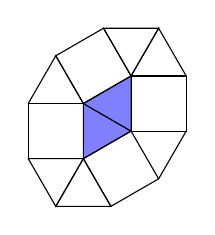
\begin{tikzpicture}[scale=0.7]
    \draw (0, 0) rectangle (1, 1);
    \draw[fill=blue!50] (1, 0)--(1,1)--({1 + sqrt(3)/2},0.5)--cycle;
    \draw[fill=blue!50] ({1 + sqrt(3)/2},1.5)--(1,1)--({1 + sqrt(3)/2},0.5)--cycle;
    \draw ({1 + sqrt(3)/2},1.5) rectangle ({2 + sqrt(3)/2},0.5);
    \draw ({1 + sqrt(3)/2},1.5)--(1,1)--(0.5, {1 + sqrt(3)/2})--({0.5 + sqrt(3)/2},{1.5 + sqrt(3)/2})--cycle;
    \draw (0,1)--(0.5, {1 + sqrt(3)/2})--(1,1);
    \draw ({1 + sqrt(3)/2},1.5)--({1.5 + sqrt(3)/2},{1.5 + sqrt(3)/2})--({2 + sqrt(3)/2},1.5)--cycle;
    \draw ({1 + sqrt(3)/2},1.5)--({0.5 + sqrt(3)/2},{1.5 + sqrt(3)/2})--({1.5 + sqrt(3)/2},{1.5 + sqrt(3)/2})--cycle;
    \draw (1, 0)--({1 + sqrt(3)/2},0.5)--({1.5 + sqrt(3)/2},{0.5 - sqrt(3)/2})--(1.5, {-sqrt(3)/2})--cycle;
    \draw (0, 0)--(0.5, {-sqrt(3)/2})--(1,0)--cycle;
    \draw (0.5, {-sqrt(3)/2})--(1,0)--(1.5, {-sqrt(3)/2})--cycle;
    \draw ({2 + sqrt(3)/2},0.5)--({1.5 + sqrt(3)/2},{0.5-sqrt(3)/2});%({2 + sqrt(3)/2},0.5);
  \end{tikzpicture}
  \\~\\
  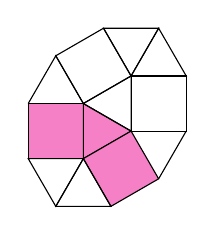
\begin{tikzpicture}[scale=0.7]
    \draw[fill=magenta!50] (0, 0) rectangle (1, 1);
    \draw[fill=magenta!50] (1, 0)--(1,1)--({1 + sqrt(3)/2},0.5)--cycle;
    \draw ({1 + sqrt(3)/2},1.5)--(1,1)--({1 + sqrt(3)/2},0.5)--cycle;
    \draw ({1 + sqrt(3)/2},1.5) rectangle ({2 + sqrt(3)/2},0.5);
    \draw ({1 + sqrt(3)/2},1.5)--(1,1)--(0.5, {1 + sqrt(3)/2})--({0.5 + sqrt(3)/2},{1.5 + sqrt(3)/2})--cycle;
    \draw (0,1)--(0.5, {1 + sqrt(3)/2})--(1,1);
    \draw ({1 + sqrt(3)/2},1.5)--({1.5 + sqrt(3)/2},{1.5 + sqrt(3)/2})--({2 + sqrt(3)/2},1.5)--cycle;
    \draw ({1 + sqrt(3)/2},1.5)--({0.5 + sqrt(3)/2},{1.5 + sqrt(3)/2})--({1.5 + sqrt(3)/2},{1.5 + sqrt(3)/2})--cycle;
    \draw[fill=magenta!50] (1, 0)--({1 + sqrt(3)/2},0.5)--({1.5 + sqrt(3)/2},{0.5 - sqrt(3)/2})--(1.5, {-sqrt(3)/2})--cycle;
    \draw (0, 0)--(0.5, {-sqrt(3)/2})--(1,0)--cycle;
    \draw (0.5, {-sqrt(3)/2})--(1,0)--(1.5, {-sqrt(3)/2})--cycle;
    \draw ({2 + sqrt(3)/2},0.5)--({1.5 + sqrt(3)/2},{0.5-sqrt(3)/2});%({2 + sqrt(3)/2},0.5);
  \end{tikzpicture}
  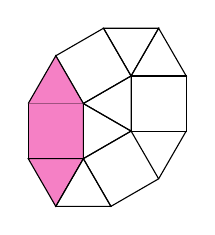
\begin{tikzpicture}[scale=0.7]
    \draw[fill=magenta!50] (0, 0) rectangle (1, 1);
    \draw (1, 0)--(1,1)--({1 + sqrt(3)/2},0.5)--cycle;
    \draw ({1 + sqrt(3)/2},1.5)--(1,1)--({1 + sqrt(3)/2},0.5)--cycle;
    \draw ({1 + sqrt(3)/2},1.5) rectangle ({2 + sqrt(3)/2},0.5);
    \draw ({1 + sqrt(3)/2},1.5)--(1,1)--(0.5, {1 + sqrt(3)/2})--({0.5 + sqrt(3)/2},{1.5 + sqrt(3)/2})--cycle;
    \draw[fill=magenta!50] (0,1)--(0.5, {1 + sqrt(3)/2})--(1,1);
    \draw ({1 + sqrt(3)/2},1.5)--({1.5 + sqrt(3)/2},{1.5 + sqrt(3)/2})--({2 + sqrt(3)/2},1.5)--cycle;
    \draw ({1 + sqrt(3)/2},1.5)--({0.5 + sqrt(3)/2},{1.5 + sqrt(3)/2})--({1.5 + sqrt(3)/2},{1.5 + sqrt(3)/2})--cycle;
    \draw (1, 0)--({1 + sqrt(3)/2},0.5)--({1.5 + sqrt(3)/2},{0.5 - sqrt(3)/2})--(1.5, {-sqrt(3)/2})--cycle;
    \draw[fill=magenta!50] (0, 0)--(0.5, {-sqrt(3)/2})--(1,0)--cycle;
    \draw (0.5, {-sqrt(3)/2})--(1,0)--(1.5, {-sqrt(3)/2})--cycle;
    \draw ({2 + sqrt(3)/2},0.5)--({1.5 + sqrt(3)/2},{0.5-sqrt(3)/2});%({2 + sqrt(3)/2},0.5);
  \end{tikzpicture}
  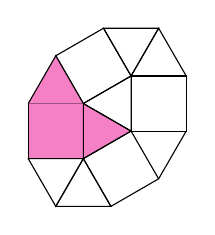
\begin{tikzpicture}[scale=0.7]
    \draw[fill=magenta!50] (0, 0) rectangle (1, 1);
    \draw[fill=magenta!50] (1, 0)--(1,1)--({1 + sqrt(3)/2},0.5)--cycle;
    \draw ({1 + sqrt(3)/2},1.5)--(1,1)--({1 + sqrt(3)/2},0.5)--cycle;
    \draw ({1 + sqrt(3)/2},1.5) rectangle ({2 + sqrt(3)/2},0.5);
    \draw ({1 + sqrt(3)/2},1.5)--(1,1)--(0.5, {1 + sqrt(3)/2})--({0.5 + sqrt(3)/2},{1.5 + sqrt(3)/2})--cycle;
    \draw[fill=magenta!50] (0,1)--(0.5, {1 + sqrt(3)/2})--(1,1);
    \draw ({1 + sqrt(3)/2},1.5)--({1.5 + sqrt(3)/2},{1.5 + sqrt(3)/2})--({2 + sqrt(3)/2},1.5)--cycle;
    \draw ({1 + sqrt(3)/2},1.5)--({0.5 + sqrt(3)/2},{1.5 + sqrt(3)/2})--({1.5 + sqrt(3)/2},{1.5 + sqrt(3)/2})--cycle;
    \draw (1, 0)--({1 + sqrt(3)/2},0.5)--({1.5 + sqrt(3)/2},{0.5 - sqrt(3)/2})--(1.5, {-sqrt(3)/2})--cycle;
    \draw (0, 0)--(0.5, {-sqrt(3)/2})--(1,0)--cycle;
    \draw (0.5, {-sqrt(3)/2})--(1,0)--(1.5, {-sqrt(3)/2})--cycle;
    \draw ({2 + sqrt(3)/2},0.5)--({1.5 + sqrt(3)/2},{0.5-sqrt(3)/2});%({2 + sqrt(3)/2},0.5);
  \end{tikzpicture}
  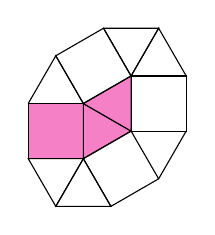
\begin{tikzpicture}[scale=0.7]
    \draw[fill=magenta!50] (0, 0) rectangle (1, 1);
    \draw[fill=magenta!50] (1, 0)--(1,1)--({1 + sqrt(3)/2},0.5)--cycle;
    \draw[fill=magenta!50] ({1 + sqrt(3)/2},1.5)--(1,1)--({1 + sqrt(3)/2},0.5)--cycle;
    \draw ({1 + sqrt(3)/2},1.5) rectangle ({2 + sqrt(3)/2},0.5);
    \draw ({1 + sqrt(3)/2},1.5)--(1,1)--(0.5, {1 + sqrt(3)/2})--({0.5 + sqrt(3)/2},{1.5 + sqrt(3)/2})--cycle;
    \draw (0,1)--(0.5, {1 + sqrt(3)/2})--(1,1);
    \draw ({1 + sqrt(3)/2},1.5)--({1.5 + sqrt(3)/2},{1.5 + sqrt(3)/2})--({2 + sqrt(3)/2},1.5)--cycle;
    \draw ({1 + sqrt(3)/2},1.5)--({0.5 + sqrt(3)/2},{1.5 + sqrt(3)/2})--({1.5 + sqrt(3)/2},{1.5 + sqrt(3)/2})--cycle;
    \draw (1, 0)--({1 + sqrt(3)/2},0.5)--({1.5 + sqrt(3)/2},{0.5 - sqrt(3)/2})--(1.5, {-sqrt(3)/2})--cycle;
    \draw (0, 0)--(0.5, {-sqrt(3)/2})--(1,0)--cycle;
    \draw (0.5, {-sqrt(3)/2})--(1,0)--(1.5, {-sqrt(3)/2})--cycle;
    \draw ({2 + sqrt(3)/2},0.5)--({1.5 + sqrt(3)/2},{0.5-sqrt(3)/2});%({2 + sqrt(3)/2},0.5);
  \end{tikzpicture}
  \caption{
    All $1$-tile, $2$-tile, and $3$-tile multipolyforms on a snub square tiling.
  }
\end{figure}
\begin{note}
  It is hard to count polyominos and polyforms more generally.
\end{note}
\begin{question}
  Is there a unified method for counting multipolyforms on an arbitrary
  tiling---that is, a method that is not \textit{ad hoc} for each tiling?
\end{question}

\begin{related}
  \item What is the smallest region of the plane that can contain all
  $k$-polyforms? (As in Moser's worm problem.)
  \item Do the multipolyforms described in the example grow significantly
  faster than polyominos? What aspects of the tiling does the asymptotic growth
  depend on?
\end{related}
\begin{references}
  \item \url{https://en.wikipedia.org/wiki/Snub_square_tiling#/media/File:1-uniform_n9.svg}
  \item \url{https://en.wikipedia.org/wiki/Euclidean_tilings_by_convex_regular_polygons}
  \item \url{https://en.wikipedia.org/wiki/Polyform}
\end{references}
\end{document}
